\documentclass[10pt,a4paper]{report}
\usepackage[utf8]{inputenc}
\usepackage[russian]{babel}
\usepackage{amsmath}
\usepackage{amsfonts}
\usepackage{amssymb}
\usepackage{graphicx}
\renewcommand{\thesection}{\arabic{section}}
\setcounter{totalnumber}{10}
\setcounter{topnumber}{10}
\setcounter{bottomnumber}{10}
\renewcommand{\topfraction}{1}
\author{Никитина Анна}
\title{Лабораторная работа №7.\\
	Сервис тестирования корректности настройки SSL на сервере Qualys SSL Labs - SSL Server Test}
\begin{document}
\maketitle
\tableofcontents
\pagebreak

\section{Цель работы}
\begin{itemize}
\item Изучить лучшие практики по развертыванию SSL/TLS.
\item Изучить основные уязвимости и атаки на SSL последнего времени - POODLE, HeartBleed.
\end{itemize}
\section{Ход работы}
\subsection{Изучение}
\subsubsection{Лучшие практики по развертыванию SSL/TLS}

SSL/TLS обманчиво кажется простой технологией. Он прост в развертывании, а потом он просто работает, не обеспечивая достаточного уровня безопасности. Но основная проблема заключается в том, что SSL/TLS нелегко правильно развернуть. Для того чтобы TLS обеспечивал необходимый уровень безопасности, системные администраторы и разработчики должны приложить дополнительные усилия в настройке своих серверов и в разработке приложений.
\begin{enumerate}
\item Приватный ключ и сертификат

Качество защиты, обеспечиваемой TLS полностью зависит от секретного ключа, закладывающего основу безопасности, и сертификата, который сообщает о подлинности сервера для его посетителей.   \\
\begin{enumerate}
\item Используйте 2048-битные закрытые ключи
\item Защитите закрытый ключ \\
 Рекомендуемые меры:
\begin{itemize}
\item Генерируйте закрытые ключи и запросы на сертификат (CSRs) на доверенном компьютере. \\
\item Используйте парольную защиту закрытых ключей, чтобы предотвратить их компрометацию в тех случаях, когда они хранятся в резервных системах. \\
\item После компрометации отзывайте старые сертификаты и генерируйте новые ключи. \\
\item Обновляйте сертификаты каждый год и всегда с новыми закрытыми ключами. \\
\end{itemize}
\item Обеспечьте охват всех используемых доменных имен
\item Приобретайте сертификаты у надежного удостоверяющего центра
\item Используйте надежные алгоритмы подписи сертификата 
\end{enumerate}

\item Конфигурация \\
Если вы правильно настроили на сервере TLS, то можете быть уверены, что данные вашего сайта корректно отображаются для посетителей сайта, используются только безопасные алгоритмы.
\begin{enumerate}
\item Используйте безопасные протоколы. К ним относятся TLS v1.0, v1.1 и v1.2 
\item Используйте безопасные алгоритмы шифрования
\item Контроль за выбором алгоритма шифрования \\
\item  Отключите Renegotiation по инициативе клиента \\
В SSL / TLS renegotiation позволяет сторонам остановить обмен данными, с тем чтобы повторно инициировать его для обеспечения безопасности. Есть некоторые случаи, в которых renegotiation должен быть инициирован сервером, но нет никакой известной необходимости позволять инициировать renegotiation клиентом. Кроме того это может облегчить организацию DDoS-атаки на ваши сервера.
\item Снижение известных проблем \\
В какой-то момент могут возникнуть проблемы с безопасностью с любым продуктом. Хорошо, если вы всегда в курсе событий в мире информационной безопасности.
\end{enumerate}
\end{enumerate}
\subsubsection{Уязвимости POODLE, HeartBleed}
\paragraph{POODLE} - это уязвимость в SSLv3, она  позволяет злоумышленнику, имеющему какую-либо возможность отправлять свои данные на сервер по SSLv3 от имени жертвы, расшифровывать по 1 байту за 256 запросов. Происходит это из-за того, что в SSLv3 не учитывается MAC адрес. \\
Теоретически, реализовать атаку POODLE можно на любой сервис, где есть возможность влиять на отправляемые данные со стороны атакуемого. Для этого атакующему необходимо: 
\begin{itemize}
\item Иметь возможность прослушивать и подменять трафик атакуемого
\item Иметь возможность совершать запросы от имени атакуемого с известным атакующему текстом
\end{itemize}
\paragraph{HeartBleed} - это уязвимость в безопасности программной библиотеки OpenSSL (открытой реализации протокола шифрования SSL/TLS), которая позволяет хакерам получить доступ к содержимому оперативной памяти серверов, в которых в этот момент могут содержаться приватные данные пользователей различных веб-сервисов. \\
Уязвимость позволяет взломщику получить доступ к 64 килобайтам оперативной памяти сервера и осуществлять атаку вновь и вновь вплоть до полной потери данных. Это означает, что утечке подвержены не только логины и пароли, но и данные файлов cookie, которые веб-серверы и сайты используют для отслеживания действий пользователя и упрощения авторизации. 
\subsection{Практическое задание}
В качестве Recent Best был проанализирован сайт forum.anfs.eu. Отчет представлен на рисунке \ref{ris:img1}. Сайт имеет оценку А. \\
\begin{figure}[ht]	\center{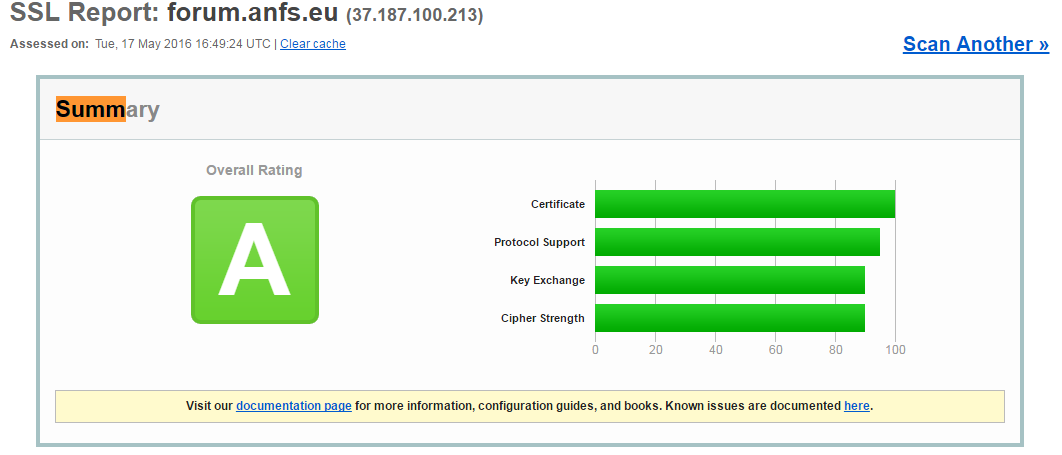
\includegraphics[width=1\linewidth]{img/1}}
\caption{Отчет для сайта forum.anfs.eu}
\label{ris:img1}
\end{figure}
В качестве Recent Worst был проанализирован сайт synata.com. Отчет представлен на рисунке \ref{ris:img2}. Сайт имеет оценку F.\\ Замечания отчета:
\begin{itemize}
\item Cайт поддерживает анонимный (небезопасный) набор алгоритмов. Оценка F.
\item Cайт поддерживает слабые Диффи-Хеллмана (DH) параметры обмена ключа. Оценка  B. 
\item Сайт поддерживает только старые протоколы, а не текущие TLS 1.2. Оценка C. 
\item Сайт принимает шифр RC4, но только с более старыми версиями протокола. Оценка В.
\item Сайт не поддерживает Forward Secrecy 
\end{itemize}
\begin{figure}[ht]	\center{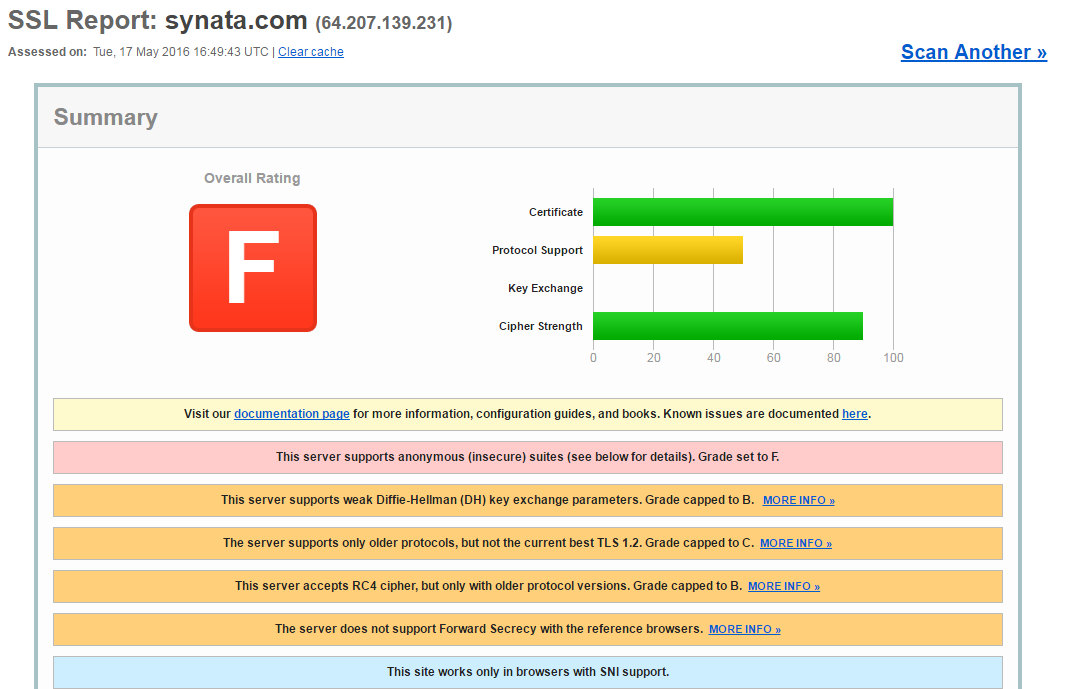
\includegraphics[width=1\linewidth]{img/2}}
\caption{Отчет для сайта synata.com}
\label{ris:img2}
\end{figure}
Выберем для самостоятельного анализа домен github.com. Домен защищен SSL шифровнием. 
\paragraph{Summary.}Отчет для выбранного домена представлен на рисунке \ref{ris:img3}. Сайт имеет оценку А+ (наивысшую). Дополнительных замечаний на домен не было обнаружено. \\
\begin{figure}[ht]	\center{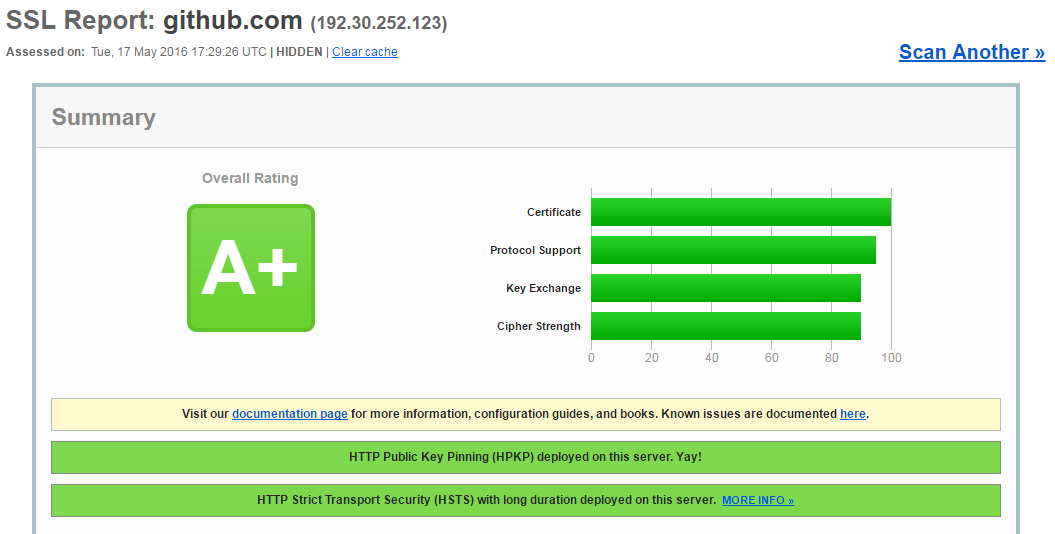
\includegraphics[width=1\linewidth]{img/3}}
\caption{Отчет для сайта github.com}
\label{ris:img3}
\end{figure}
\paragraph{Configuration.}Расшифруем шифры в этом разделе.
\begin{verbatim}
TLS_ECDHE_RSA_WITH_AES_128_GCM_SHA256 (0xc02f)   ECDH secp256r1 (eq. 3072 bits RSA)   FS	128
TLS_ECDHE_RSA_WITH_AES_256_GCM_SHA384 (0xc030)   ECDH secp256r1 (eq. 3072 bits RSA)   FS	256
TLS_ECDHE_RSA_WITH_AES_128_CBC_SHA256 (0xc027)   ECDH secp256r1 (eq. 3072 bits RSA)   FS	128
TLS_ECDHE_RSA_WITH_AES_128_CBC_SHA (0xc013)   ECDH secp256r1 (eq. 3072 bits RSA)   FS	128
TLS_ECDHE_RSA_WITH_AES_256_CBC_SHA384 (0xc028)   ECDH secp256r1 (eq. 3072 bits RSA)   FS	256
TLS_ECDHE_RSA_WITH_AES_256_CBC_SHA (0xc014)   ECDH secp256r1 (eq. 3072 bits RSA)   FS	256
TLS_RSA_WITH_AES_128_GCM_SHA256 (0x9c)	128
TLS_RSA_WITH_AES_256_GCM_SHA384 (0x9d)	256
TLS_RSA_WITH_AES_128_CBC_SHA256 (0x3c)	128
TLS_RSA_WITH_AES_128_CBC_SHA (0x2f)	128
TLS_RSA_WITH_AES_256_CBC_SHA256 (0x3d)	256
TLS_RSA_WITH_AES_256_CBC_SHA (0x35)	256
\end{verbatim}
\begin{itemize}
\item TLS - протокол защищенной передачи данных;
\item ECDHE - алгоритм Диффи-Хэлмана на эллиптических кривых;
\item RSA - алгоритм шифрования с открытым ключем;
\item GCM - режим блочного шифрования;
\item CBC - режим блочного шифрования;
\item AES\_128 - алгоритм шифрования с длиной ключа в 128 бит;
\item SHA256 - хэш-функция с длиной ключа 256 бит;
\item SHA384 - хэш-функция с длиной ключа 384 бит.
\end{itemize}
\paragraph{Protocol Details.} Просмотрим детали протокола подробнее   \\
Сайт защищен от атак DROWN, BEAST, POODLE (SSLv3, TLS)
\begin{verbatim}
DROWN (experimental)	No, server keys and hostname not seen elsewhere with SSLv2
BEAST attack	Not mitigated server-side (more info)   TLS 1.0: 0xc013
POODLE (SSLv3)	No, SSL 3 not supported (more info)
POODLE (TLS)	No (more info)
\end{verbatim}
Поддерживается технология привязки ключей
\begin{verbatim}
Public Key Pinning (HPKP)	Yes
\end{verbatim}
Сайт поддерживает функцию Heartbeat, но защищен от уязвимости Heartbleed, основанной на этой функции.
\begin{verbatim}
Heartbeat (extension)	Yes
Heartbleed (vulnerability)	No (more info)
\end{verbatim}
Поддержка Forward Security для современных браузеров.
\begin{verbatim}
Forward Secrecy	With modern browsers (more info)
\end{verbatim}
Поддерживает ALPN и не поддерживает NPN.
\begin{verbatim}
ALPN	Yes
NPN	No
\end{verbatim}
Поддержка возобновления сессии, используя механизм кеширования.
\begin{verbatim}
Session resumption (caching)	Yes
Session resumption (tickets)	No
\end{verbatim}
Перенаправление на HTTPS при помощи HSTS
\begin{verbatim}
Strict Transport Security (HSTS)	Yes 
HSTS Preloading
\end{verbatim}
Предотвращение атаки Downgrade attack, с помощью которой злоумышленник может понизить версию используемых протоколов.
\begin{verbatim}
Downgrade attack prevention	Yes, TLS_FALLBACK_SCSV supported
\end{verbatim}
Протокол Диффи-Хеллмана не поддерживается.
\begin{verbatim}
Uses common DH primes	No, DHE suites not supported
DH public server param (Ys) reuse	No, DHE suites not supported
\end{verbatim}
\paragraph{Итоговый вывод.} Домен github.com имеет наивысшую оценку (А+) по реализации SSL. Сайтом поддерживается технология привязки ключей, функция Heartbeat( при этом осуществлена защита от уязвимости Heartbleed, основанной на этой функции). Также поддерживаются: Forward Security для современных браузеров, ALPN, возможность возобновления сессии при помощи механизма кеширования и другое. Данный домен является надежным.
\section{Вывод}
В ходе данной лабораторной работы были изучены возможности сервиса SSL Labs, анализирующего качество защиты домена. \\
Были просмотрены отчеты для двух типов сервисов: имеющих наибольшую оценку и наименьшую. \\
Также был проанализирован домен github.com. Был просмотрен отчет по данному домену, содержащий конкретные детали: используемые способы шифрования, защита от уязвимстей и другое. На основе полученной информации был сделан вывод, что сайт github.com является хорошо защищенным.
\end{document}
